\documentclass{jarticle}

\usepackage{graphicx}
\usepackage{url}
\usepackage{listings,jlisting}
\usepackage{ascmac}
\usepackage{amsmath,amssymb}

%ここからソースコードの表示に関する設定
\lstset{
    basicstyle={\ttfamily},
    identifierstyle={\small},
    commentstyle={\smallitshape},
    keywordstyle={\small\bfseries},
    ndkeywordstyle={\small},
    stringstyle={\small\ttfamily},
    frame={tb},
    breaklines=true,
    columns=[l]{fullflexible},
    numbers=left,
    xrightmargin=0zw,
    xleftmargin=3zw,
    numberstyle={\scriptsize},
    stepnumber=1,
    numbersep=1zw,
    lineskip=-0.5ex
}
%ここまでソースコードの表示に関する設定 

\title{知能プログラミング演習II 課題2}
\author{グループ07\\
    29114007 池口 弘尚\\
    29114031 大原 拓人\\
    29114048 北原 太一\\
    29114086 飛世 裕貴\\
    29114095 野竹 浩二朗\\
%  {\small (グループレポートの場合は、グループ名および全員の学生番号と氏名が必要)}
}
\date{2019年10月7日}

\begin{document}
\maketitle

\paragraph{提出物} rep1 group07.zip
\paragraph{グループ} グループ07

\section{課題の説明}
\begin{description}
    \item[必須課題2-1] MatchingクラスまたはUnifyクラスを用い,パターンで検索可能な簡単なデータベースを作成せよ.
    与えられたパターンにマッチする全データを列挙するプログラムを作成せよ.
    \\ 例えば,この例のような形式のデータセットから,?x has a hobby of playing video-games や 
    Hanako is a ?y のような,様々なパターンにマッチするデータを検索できるようにすること.
    複数のパターンが与えられたときに全ての可能な変数束縛の集合を返すようなプログラムを作成せよ.
    \\ 例えば,上記の例で「?x is a boy」と「?x loves ?y」の両方が与えられたときに,(?x, ?y) の
    全ての可能な変数束縛の集合として{(Taro, Jiro), (Jiro, Hanako)}を返すこと.
    \item[必須課題2-2] 自分たちの興味ある分野の知識についてデータセットを作り,上記2-1で実装したデータベースに登録せよ.
    また,検索実行例を示せ.どのような方法でデータセットを登録しても構わない.
    \item[発展課題2-3] 上記システムのGUIを作成せよ.
    \\ データの追加,検索,削除をGUIで操作できるようにすること.
    \\ 登録されたデータが次回起動時に消えないよう,登録されたデータをファイルへ書き込んだり読み込んだりできるようにすること.
\end{description}


\section{課題2-1}
\begin{screen}
    MatchingクラスまたはUnifyクラスを用い,パターンで検索可能な簡単なデータベースを作成せよ.
    与えられたパターンにマッチする全データを列挙するプログラムを作成せよ.
    \\ 例えば,この例のような形式のデータセットから,?x has a hobby of playing video-games や 
    Hanako is a ?y のような,様々なパターンにマッチするデータを検索できるようにすること.
    複数のパターンが与えられたときに全ての可能な変数束縛の集合を返すようなプログラムを作成せよ.
    \\ 例えば,上記の例で「?x is a boy」と「?x loves ?y」の両方が与えられたときに,(?x, ?y) の
    全ての可能な変数束縛の集合として{(Taro, Jiro), (Jiro, Hanako)}を返すこと.
\end{screen}
\subsection{手法}
    配列にデータベース用の文字列を格納し、for文を用いて配列の中を走査するようにした。
    統合開発環境を用いているため、コマンドライン引数の変更の手間が省けるように、
    入力ストリームから検索するパターンを読み込むように変更した。
    検索の効率をよくするためにDataBaseクラスのSearchメソッドで絞り込みを行ってから、走査するようにした。
    複数のパターンを読み込めるようにし、変数束縛の集合と一致したパターンの数を引数で渡しつつ、
    再帰アルゴリズムを用いて検索するsearchメソッドを作成した。
\subsection{実装-29114031 大原 拓人}
    もともと与えられたUnify.javaを以下のように変更した。
    \paragraph{}
    まず、コマンドライン引数で使用するデータセットを読み込む。
    読み込みが完了したら、検索するパターンを入力するように促して
    入力ストリームからパターンを読み取る。読み取ったパターンは、
    Unifierインスタンスを作成し、そのsearchメソッドの引数として渡す。

\begin{lstlisting}[caption=Unifyクラスより抜粋]
public static void main(String arg[]) {
// For CUI Test
Scanner stdin = new Scanner(System.in);
    for (int i = 0; i < arg.length; i++) {
        try {
            BufferedReader reader = new BufferedReader(new InputStreamReader(new FileInputStream(arg[i]), "UTF-8"));
            String s = reader.readLine();
            while (s != null) {
                if (!s.equals(""))
                    DataBase.getDataBase().insert(s);
                s = reader.readLine();
            }
            reader.close();
        } catch (UnsupportedEncodingException e) {
            // TODO Auto-generated catch block
            e.printStackTrace();
        } catch (FileNotFoundException e) {
            // TODO Auto-generated catch block
            e.printStackTrace();
        } catch (IOException e) {
            // TODO Auto-generated catch block
            e.printStackTrace();
        }
    }
    while (true) {
        System.out.println("Enter Search Pattern:");
        String scan = stdin.nextLine();
        if (scan.equals("exit"))
            break;
        (new Unifier()).search(scan);
        for (String string : Unifier.getMatchList())
            System.out.println(string);
        for (String string : Unifier.getVarSets())
            System.out.println(string);
    }
    stdin.close();
}
\end{lstlisting}
    \paragraph{}
    絞り込みで得られたデータを使い回すためにstatic変数としている。
    また、マッチングに成功したときのデータと変数束縛の集合も
    探索後に消えてしまわないように、static型に格納して後から
    アクセスできるようにした。マッチングを始める前に、
    これらのstatic変数は初期化される。
\begin{lstlisting}[caption=Unifierクラスの主要パーツ]
class Unifier {
    private static DataBase[] results;
    private static String[] terms;
    private static ArrayList<String> varSets;
    private static ArrayList<String> matchList;
    ...
    //ここでそのほかの変数、コンストラクタ、セッタ、ゲッタなどを定義
    ...

    public static void setByTerms(String str) {
        // 検索するパターンをもとにDataBaseクラスのSearchメソッドで絞り込み格納
        String[] terms = str.split(";");
        Unifier.terms = terms;
        DataBase[] results = new DataBase[terms.length];
        for (int i = 0; i < results.length; i++) {
            results[i] = DataBase.getDataBase().Search(terms[i]);
        }
        Unifier.results = results;
    }

    private static void addMatchList(ArrayList<String> matched) {
        // 重複するものは加えない
        for (String addline : matched) {
            boolean match = false;
            for (String string : Unifier.matchList) {
                if (addline.equals(string)) {
                    match = true;
                    break;
                }
            }
            if (!match)
                Unifier.matchList.add(addline);
        }
    }

    public boolean search(String str) {
        // 結果の初期化
        cleanVarSets();
        cleanMatchList();
        setByTerms(str);
        return search(new HashMap<>(), new ArrayList<>(), 0);
    }
    ...
\end{lstlisting}
    \paragraph{}
    それまでに得られた変数束縛の組と、マッチしたパターンの組、何個目の式の
    マッチングかを表す整数を引数として、再帰アルゴリズムを用いて実装した。
    一つでもマッチする組み合わせがあれば、trueを返す。
\begin{lstlisting}[caption=searchメソッド]
...
boolean search(HashMap<String, String> vars, ArrayList<String> matched, int layer) {
    // 再帰でバックトラック可能に
    boolean match = false;
    if (layer < terms.length) {
        if (Unifier.results[layer] == null)
            return false;
        Unifier unifier = new Unifier(Unifier.results[layer].GetResult());
        for (String string : unifier.lines) {
            unifier.setVars(vars);
            unifier.setMatched(matched);
            if (unifier.unify(string, terms[layer])) {
                unifier.matched.add(string);
                match = search(unifier.vars, unifier.matched, layer + 1) || match;
            }
        }
    } else {
        // すべての層(パターン式)を通過すれば結果に追加
        addMatchList(matched);
        String varset = vars.toString();
        for (String string : matched)
            // マッチした文を結果に追加
            addVarSets(string);
        if (varset.equals("{}"))
            // 変数がなければtrue.
            addVarSets("true.");
        else
            addVarSets(varset);
        return true;
    }
    return match;
}
...
\end{lstlisting}

\subsection{実行例-29114031 大原 拓人}
ここではmoodleで与えられたデータセットの例を用いた。
\begin{lstlisting}[caption=Unify.javaの実行例]]
Enter Search Pattern:
Taro is a boy
Taro is a boy
true.
Enter Search Pattern:
?x is a boy  
Taro is a boy
{?x=Taro}
Jiro is a boy
{?x=Jiro}
Enter Search Pattern:
?x loves ?y;?y loves ?z;?z loves ?x
Hanako loves Taro
Taro loves Jiro
Jiro loves Hanako
{?x=Hanako, ?y=Taro, ?z=Jiro}
Taro loves Jiro
Jiro loves Hanako
Hanako loves Taro
{?x=Taro, ?y=Jiro, ?z=Hanako}
Jiro loves Hanako
Hanako loves Taro
Taro loves Jiro
{?x=Jiro, ?y=Hanako, ?z=Taro}
Enter Search Pattern:
exit
\end{lstlisting}
    \paragraph{}
    変数がなければ、「true.」が表示される。
    複数のパターンをセミコロン「;」で区切って入力することでそれらの検索ができ、
    一致したパターンとその時の変数束縛の集合が表示されている。

\subsection{考察-29114031 大原 拓人}
もともと入力されたパターンごとにデータセットを全走査する予定だったが、
グループの池口君が絞り込みにかなり有効なDataBaseクラスを作ってくれたので、
探索の効率がかなり向上した。変数束縛の組を共有せず、インスタンスごとに
複製して引き継ぐことで、バックトラックらしい挙動を再現できた。

\subsection{実装-29114007 池口 弘尚}
まず、新たに追加したクラスは以下の
\begin{itemize}
\item DataBaseクラス: 読み込んだ文字列をDataクラスとして保持しておくためのクラス。文字列の具体化されている部分から候補を絞る機能も持つ。
\item Dataクラス: 最初の名詞が同じものの文字列を保存しておくためのクラス。
\item SentenceAnalysisクラス: 文字列を最初の名詞と動詞周辺とそれ以外に分けるためのクラス。
\item Unifierクラス: 具体化されていない文字列を使用して探索を行うクラス。
\end{itemize}

SentenceAnalysisクラスにおける文字列を三分割するためのメソッドAnalysisは以下のように実装した。

\begin{lstlisting}[caption=SentenceAnalysisのAnalysis,label=src:Analysis]
static String[] Analysis(String sentence) throws NoSuchElementException {
	String[] elements = new String[3];
	StringTokenizer tokenizer = new StringTokenizer(sentence);
	elements[0] = tokenizer.nextToken();
	elements[1] = tokenizer.nextToken();
	elements[2] = "";
	while (true) {
		String t = tokenizer.nextToken();
        //前置詞が含まれていた場合はそれ以前を動詞部分に結合
		if (PrepositionCheck(t)) {
			if (elements[2] == "")
				elements[1] += " " + t;
			elements[2] += t;
			elements[1] += " " + elements[2];
			elements[2] = "";
		} else {
			elements[2] += t;
			if (tokenizer.hasMoreTokens())
				elements[2] += " ";
			else
				break;
		}
	}
	return elements;
}
\end{lstlisting}


Dataクラスは同じ名詞のデータを格納する機能を持っている。データの操作に関するinsert,remove,searchは以下のように実装した。
\begin{lstlisting}[caption=Dataのデータ操作関連のメソッド,label=src:DataControl]
//メンバ変数として持つ名詞部分とそれ以降
String name;
Map<Integer, List<String>> records;

//コンストラクタで名詞を設定
public Data(String name) {
	this.name = name;
	records = new HashMap<>();
}

//要素を追加
public void insert(int key, String value) {
	if (records.containsKey(key)) {
		records.get(key).add(value);
	} else {
		List<String> list = new ArrayList<>();
		list.add(value);
		records.put(key, list);
	}
}

//要素を削除
public boolean remove(int key, String value) {
	boolean result = false;
	List<String> list = records.get(key);
	if (list != null) {
		result = list.remove(value);
        //空になったらマップを削除
		if (list.isEmpty())
			records.remove(key);
	}
	return result;
}

//動詞付近で検索
public boolean Search(Collection<Integer> collection) {
	for (Integer integer : collection) {
		if (records.containsKey(integer))
			return true;
	}
	return false;
}

//後部で検索
public boolean Search(String value) {
	for (List<String> list : records.values()) {
		for (String s : list) {
			if (s==value)
				return true;
		}
	}
	return false;
}
\end{lstlisting}

上記のDataクラスを利用して、データを格納するクラスDataBaseクラスを実装してある。
DataBaseは常に自身のインスタンスを保持する。それを以下のように実装した。
\begin{lstlisting}[caption=DataBaseのインスタンス保持,label=src:DataBaseInstance]
public class DataBase {
	private static DataBase instance = new DataBase();
	Map<String, Data> datas;
	Map<String,Integer> keyMap;
	static int id = 0;

	//常に同じインスタンスを返す
	static DataBase getDataBase() {
		return instance;
	}
    ...
}
\end{lstlisting}

また、DataBaseのデータの操作に関するinsert,remove,searchは以下のように実装した。
\begin{lstlisting}[caption=DataBaseのデータ操作,label=src:DataBase]
//文の追加
boolean insert(String sentence) {
	String[] values = null;
    //具体化されていないものは読み込まない
	if(sentence.contains("?"))
		return false;
	try {
		values = SentenceAnalysis.Analysis(sentence);
	} catch (Exception e) {
		return false;
	}
	int key = -1;
	if (!keyMap.containsKey(values[1])) {
		keyMap.put(values[1],id++);
		key = keyMap.size() - 1;
	} else
		key = keyMap.get(values[1]);
	if (datas.containsKey(values[0])) {
		datas.get(values[0]).insert(key, values[2]);
	} else {
		Data data = new Data(values[0]);
		data.insert(key, values[2]);
		datas.put(values[0], data);
	}
	return true;
}

//文の削除
boolean remove(String sentence) {
	String[] values = null;
	try {
		values = SentenceAnalysis.Analysis(sentence);
	} catch (Exception e) {
		return false;
	}

	int key = keyMap.get(values[1]);
	if (key != -1) {
		Data data = datas.get(values[0]);
		if (data.remove(key, values[2])) {
			if (data.records.isEmpty())
				datas.remove(values[0]);
			return true;
		}
	}
	return false;
}

//名詞部分で候補を絞る
DataBase searchByName(String name) {
	DataBase dataBase = new DataBase();
    //データのインスタンスは作成しない
	Data d = datas.get(name);
	if (d == null)
		return null;
	Set<Integer> keyset =d.records.keySet();
	for (String s : keyMap.keySet()) {
		if(keyset.contains(keyMap.get(s)))
			dataBase.keyMap.put(s, keyMap.get(s));
	}
	dataBase.datas.put(name, d);
	return dataBase;
}

//文で検索
DataBase Search(String sentence) {
	DataBase dataBase = this;
	String[] values = null;
	try {
		values = SentenceAnalysis.Analysis(sentence);
	} catch (Exception e) {
		return null;
	}
    //具体化されている部分から候補を絞る
	if (!isVar(values[0]))
		dataBase = dataBase.searchByName(values[0]);
	if (!isContainVar(values[1]))
		dataBase = dataBase.searchByVarb(values[1]);
	if (!isContainVar(values[2]))
		dataBase = dataBase.searchByValue(values[2]);
	return dataBase;
}
\end{lstlisting}

\subsection{実行例-29114007 池口 弘尚}
追加したデータ

Hanako is a girl

Jiro loves Hanako


検索した文字列

?x is a girl;?z loves ?x

\{?x=Hanako, ?z=Jiro\}


削除した文字列

Jiro loves Hanako

検索した文字列

?x is a girl;?z loves ?x

検索失敗
\subsection{考察-29114007 池口 弘尚}
データベースに関しては、全体として1つしか実体を持たないため、疑似シングルトンパターンを使用した。
これは、候補を絞るときにDataBaseそのものを返した方が都合が良いためそのような実装となった。
DataBaseの特徴としては、文を三分割して保存するということもそうだが、最も気を付けて作った部分は検索するときにDataのインスタンスに手を加えないことによって、Dataを新しく作らなくても絞った後のDataBaseを形成することができるという点である。
DataBaseのインスタンスを作成したとしても、Dataを使いまわしていればメモリの消費を抑えることができる。

絞り込むプロセスとしては、三分割した中で具体化されている部分のみを使用して絞り込んでいる。
しかし、実際にはこのプロセスで文全体を一度見回しているため、この段階で具体化もしておいた方がより効率よく探索できると考えられる。

また、最後の部分での絞り込みにおいては、Dataの中身を変えることができないため、十分に絞ることができなかった。
これはSearchがDataBase型で返しているために実装ができなくなってしまうが、List<String>で返すことによって解決できる可能性がある。


\section{課題2-2}
\begin{screen}
    自分たちの興味ある分野の知識についてデータセットを作り,上記2-1で実装したデータベースに登録せよ.
    また,検索実行例を示せ.どのような方法でデータセットを登録しても構わない.
\end{screen}

\subsection{手法}
用意したデータセット"Dataset.txt"は「大乱闘スマッシュブラザーズスペシャル」に登場するキャラクター79体のデータである。性別や種族、元のゲームのデータなどが記されている。

\subsection{実行例-29114095 野竹浩二朗}
実行結果のすべてを載せてしまうと長くなってしまうため、自分が与えたパターンと検索に引っかかったキャラクターのみを何パターンか記す。
\\
\begin{table}[ht]
\begin{tabular}{|c|l|}
\hline
\multicolumn{1}{|l|}{与えたパターン} & \multicolumn{1}{c|}{検索結果} \\ \hline
?x is female & \begin{tabular}[c]{@{}l@{}}ロゼッタ\&チコ・サムス・パルテナ・ベヨネッタ・ピーチ・ゼロスーツサムス\\ デイジー・しずえ・ダークサムス・ルキナ・ゼルダ\end{tabular} \\ \hline
?x use a gun & サムス・ベヨネッタ・ゼロスーツサムス・ダークサムス \\ \hline
?x has wings & ベヨネッタ \\ \hline
\end{tabular}
\end{table}
\\
1つ目のパターンで女性キャラクター、2つ目で銃を使うキャラクター、3つ目で羽が生えているキャラクターを検索している。この条件に合うキャラクターはベヨネッタだけなのでしっかりと検索出来ている。\\

\begin{table}[ht]
\begin{tabular}{|c|l|}
\hline
\multicolumn{1}{|l|}{与えたパターン} & \multicolumn{1}{c|}{検索結果} \\ \hline
?x is gender-unknown & \begin{tabular}[c]{@{}l@{}}ヨッシー・ミュウツー・カムイ・WiiFitTrainer・ゲッコウガ・プリン\\ インクリング・ピチュー・ルカリオ・シーク・Mii-Fighter・ピカチュー\\ パックンフラワー・アイスクライマー・メタナイト・ガオガエン\\ Mr.Game\&Watch・リドリー・ヒーロー・ロックマン・むらびと\\ カービィ・ロボット・パックマン\end{tabular} \\ \hline
\begin{tabular}[c]{@{}c@{}}?x is a character of \\ KIRBY'S-DREAM-LAND\end{tabular} & カービィ・メタナイト \\ \hline
?x is pink & カービィ \\ \hline
\end{tabular}
\end{table}
1つ目の要素では"性別不明"を検索しているが、設定として性別が分からないキャラだけでなく、ポケモンなど両方があり得る場合や、アイスクライマーなど2人で一つのキャラクターとなっている場合も検索対象となっている。

\begin{table}[ht]
\begin{tabular}{|c|l|}
\hline
\multicolumn{1}{|l|}{与えたパターン} & \multicolumn{1}{c|}{検索結果} \\ \hline
?x is male & 男性キャラ多数のため省略 \\ \hline
?x has ?y & \begin{tabular}[c]{@{}l@{}}ブラックピット・スネーク・ルイージ・ドンキーコング・ソニック・マリオ\\ フォックス・ネス・ファルコ・ディディーコング・ワリオ・ピット・ルフレ\end{tabular} \\ \hline
?x is an angel & ピット・ブラックピット \\ \hline
\end{tabular}
\end{table}
1つ目のパターンで男性キャラクターを検索しているが、多数ヒットするため省略した。2つ目では何かを持っているキャラクターを検索したが、単に道具だけでなく、翼などの身体的特徴も"has"を用いて表現したため、ここでも多数のキャラクターがヒットしている。


\subsection{考察-29114095 野竹浩二朗}
3通りの検索結果を載せたが、3パターンとも思ったように検索できていることが分かった。\\
データセットの書き方がすべてのキャラクターで"X is Y"という書き方を含んでいるため、"?x is ?y"というパターンを与えても何の意味もない。また使っている動詞もワンパターンとなってしまっているので、キャラクターを絞るには具体的なキャラクター名や、ゲーム名が必要である。\\
様々なゲームのキャラクター同士を戦わせるというゲームである都合上、キャラクター同士の関係性がほぼなく、データセットの例にあった"?x loves ?y"といったパターンで検索することが難しかった。\\
79体という少なくないキャラクターの中から特定のパターンを検索する場合、もっと多くの特徴や、他キャラクターとの関係が記述されたデータセットを用意しなければならない。

\subsection{実装-29114048 北原 太一}
データセットは、3名で作成したが、監視の有無や使う単語などの統一を図った。具体的な内容については、Dataset.txtを参照されたい。

\subsection{考察-29114048 北原 太一}
今回は1人が作成したcsvライクなファイルからデータセットを手動で生成したが、何かしらのプログラムにより自動化すれば効率的に文を生成でき、残りの課題の高クォリティ化に繋がったかもしれない。
\subsection{実装-29114086 飛世裕貴}
上記したデータセットのデータベースへの登録はDataset.txtを読み込み、各データを課題2-1で実装したDataBaseクラスのインスタンスとして挿入していくことで実装した。
\subsection{実行例-29114086 飛世裕貴}
データベースへ登録したデータに対して検索を行なった結果の一部を以下に示す。
\\

\begin{screen}
\begin{verbatim}
Enter Search Pattern:
?x is male
…  (中略)
Black-Pit is male
{?x=Black-Pit}
Pikmin&Olimar is male
{?x=Pikmin&Olimar}
ToonLink is male
{?x=ToonLink}
DonkeyKong is male
{?x=DonkeyKong}
…(以下略)
\end{verbatim}
\end{screen}
\\

このように検索した結果、該当したデータと変数束縛の集合が表示されていることが確認できる。またここでは示していないが、「?x is ?y」や「?x has ?y」といった検索語においても検索を行なった結果、同様に該当したデータと変数束縛の集合が表示されることを確認した。
\subsection{考察-29114086 飛世裕貴}
今回の課題において「A is B」や「C has D」という形式のデータを扱ったが、キャラクター同士の関係性が希薄であったため、各データの関連性が小さいものとなってしまった。また今回の課題では入力したデータをただの文字列として扱っていたために「Jiro loves Hanako」のように互いの関係性を表すデータが入力されたとしても、真に登場人物間の関係性を考慮するデータ構造を実現することが出来ず、検索して初めて関係性が決定するというものとなった。
今回のようにテキストデータを扱う場合はそのデータに対して形態素解析を行い、動詞のような各登場人物間の関係性を表す単語をキーとして保存しておくことで、関係性を考慮したデータ構造を取るリレーショナルデータベースを構築できると考える。

\section{課題2-3}
\begin{screen}
    課題2-1で作成したシステムのGUIを作成せよ.
    \\ データの追加,検索,削除をGUIで操作できるようにすること.
    \\ 登録されたデータが次回起動時に消えないよう,登録されたデータをファイルへ書き込んだり読み込んだりできるようにすること.
\end{screen}
\subsection{手法}
swingのカードレイアウトを使用して、それぞれの機能をパネル分けし、大きなパネルで扱うことができるように実装した。

\subsection{実装-29114007 池口 弘尚}
まず、新たに追加したクラスは以下の
\begin{itemize}
\item FrameBaseクラス: JFrameを継承。コンストラクタのみ実装しており、JFrameの各種設定が1行でできるようにしてある。rep1と同じ。
\item MakeGUIFrameクラス: GUIの型を作成するためのクラス。
\item AddPanel,SearchPanel,RemovePanelクラス: JPanelを継承。各種パネルを描画するためのメソッドが実装されている。
\item TextLogクラス: JScrollPaneを継承。ビューポートにJTextAreaを持ち、ログを表示するためのクラス。
\item TxtFilterクラス: FileFilterを継承。JFileChooserのフィルタ。
\end{itemize}

MakeGUIFrameにおけるカードレイアウトは以下のように実装した。


\begin{lstlisting}[caption=GUI作成,label=src:MakeGUIFrame]
public static void MakeMatchingGUI() {
	FrameBase frame = new FrameBase("test", 1000, 500);
	JPanel cardPanel;
	CardLayout layout;
	/* カード1 */
	AddPanel card1 = new AddPanel();

	/* カード2 */
	SearchPanel card2 = new SearchPanel();

	/* カード3 */
	RemovePanel card3 = new RemovePanel();

	//cardPanelにカードレイアウトをセット
	cardPanel = new JPanel();
	layout = new CardLayout();
	cardPanel.setLayout(layout);

	cardPanel.add(card1, "Add");
	cardPanel.add(card2, "Search");
	cardPanel.add(card3, "Remove");

	ActionListener listener = new ActionListener() {

		@Override
		public void actionPerformed(ActionEvent e){
			String cmd = e.getActionCommand();

			switch (cmd) {
			case "Add":
			case "Search":
			case "Remove":
            	//ページの切り替え
				layout.show(cardPanel, cmd);
				break;
			case "Save":
				Save(frame);
				break;
			case "Exit":
				System.exit(0);
				break;
			default:
				System.out.println("ボタンの割り当てが存在しない");
				break;
			}
		}
	};
    ...
}
\end{lstlisting}

カードパネルに乗せるパネルであるAddPanel,SearchPanel,RemovePanelの基本的な構造は同じで、ボタンをクリックしたときに、テキストボックスに入れられた文字を読み取って処理するだけなので説明は省く。
ただ、AddPanelにはファイルを参照して読み込む機能が以下のように実装されている。
\begin{lstlisting}[caption=ファイルの参照,label=src:FileChooser]
//参照ボタンのActionListener
ActionListener listener2 = new ActionListener() {

	@Override
	public void actionPerformed(ActionEvent e) {
    	//カレントディレクトリのパスを得る
		String path = System.getProperty("user.dir");
		JFileChooser filechooser = new JFileChooser(path);
        //フィルタを追加
		filechooser.setFileFilter(new TxtFilter());
		int selected = filechooser.showOpenDialog(p2);
		if (selected == JFileChooser.APPROVE_OPTION) {
			File file = filechooser.getSelectedFile();
			adress.setText(file.getAbsolutePath());
		}
	}
};
\end{lstlisting}

また、それぞれのパネルでのログを表示するためにTextLogを以下のように実装した。
\begin{lstlisting}[caption=TextLog,label=src:TextLog]
class TextLog extends JScrollPane {
	JTextArea area;
	JViewport viewport;

	public TextLog(int rows, int columns) {
		super();
		area = new JTextArea(rows, columns);
		EtchedBorder border = new EtchedBorder(EtchedBorder.RAISED);
		area.setEditable(false);
		area.setBorder(border);
		setViewportView(area);
		viewport = getViewport();
	}

	//ログを1行分書き込む
	public void addLog(String txt) {
		area.append(txt + "\n");
	}
}
\end{lstlisting}



\subsection{実行例-29114007 池口 弘尚}
実行すると次のようなGUIが表示される。


\begin{figure}[!hbt]
  \centering
  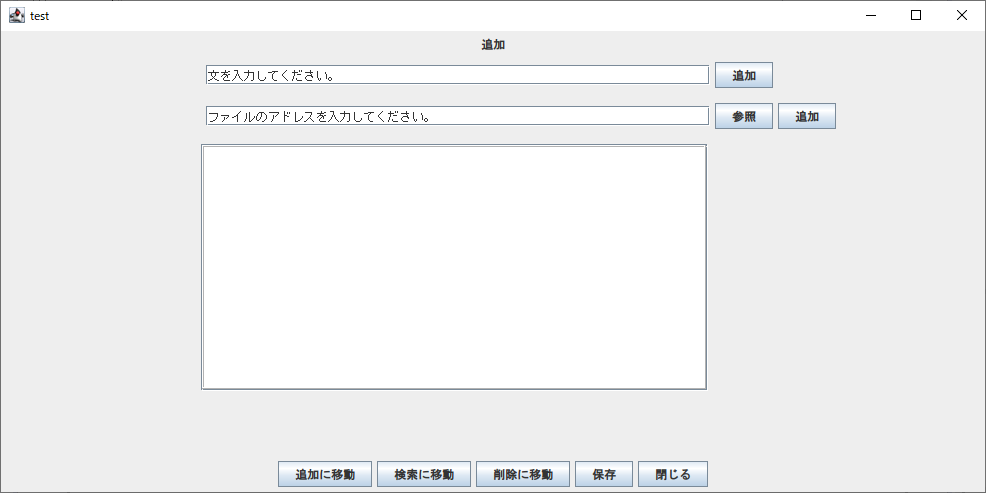
\includegraphics[bb=0 0 986 493,width=1.2\linewidth]{pic1.png}
  \caption{追加のGUIパネル}
  \label{fig:pic1}
\end{figure}

上のテキストボックスを利用すれば、1文ずつデータベースに追加することができる。下の参照をクリックすると次のように表示される。

\begin{figure}[!hbt]
  \centering
  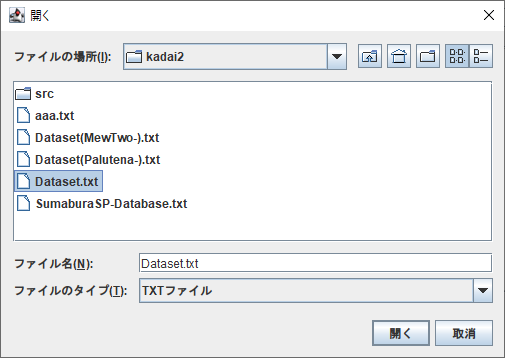
\includegraphics[bb=0 0 505 358,width=1\linewidth]{pic2.png}
  \caption{読み込むファイルを参照}
  \label{fig:pic2}
\end{figure}

これでデータセットの.txtを開くと自動的にpathが入力され、追加を押せばデータセットを読み取ってくれる。

検索パネルでは、検索する文を;で区切って入力することによって複数の文を検索することができる。

\begin{figure}[!hbt]
  \centering
  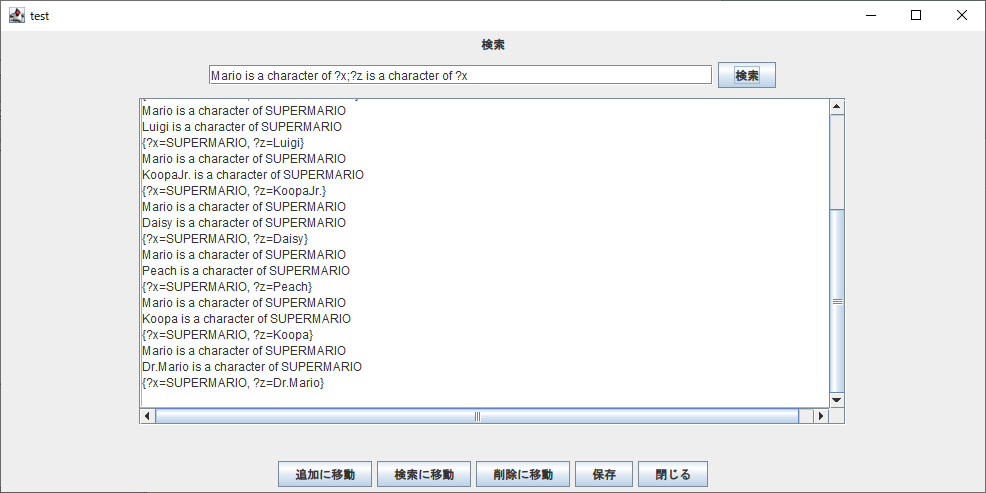
\includegraphics[bb=0 0 986 493,width=1.2\linewidth]{pic4.png}
  \caption{検索のGUIパネル}
  \label{fig:pic4}
\end{figure}

削除パネルでは入力した文をデータベースから取り除くことができる。また、検索時のように具体化されていない値を用いることによって一括で削除することもできる。

\begin{figure}[!hbt]
  \centering
  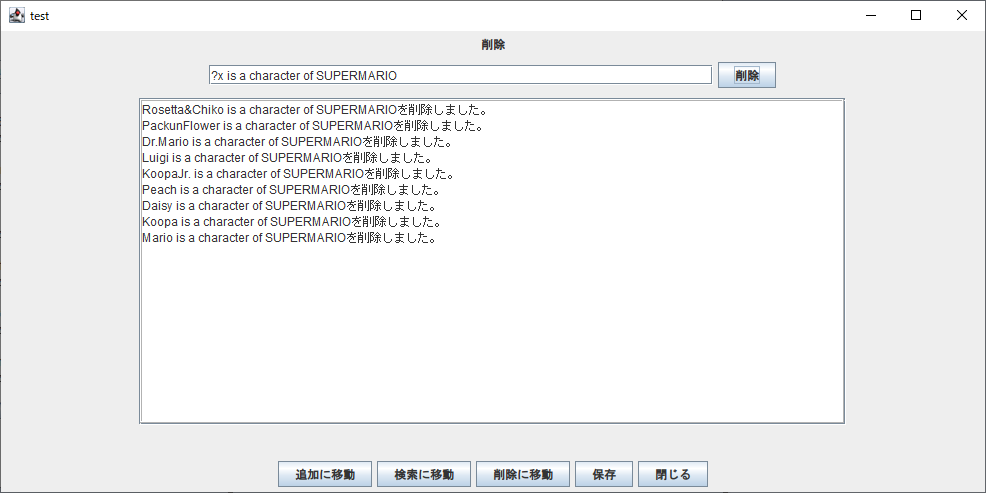
\includegraphics[bb=0 0 986 493,width=1.2\linewidth]{pic5.png}
  \caption{削除のGUIパネル}
  \label{fig:pic5}
\end{figure}

また、保存ボタンを押すと現在のデータベースを.txtで保存することができる。
\begin{figure}[!hbt]
  \centering
  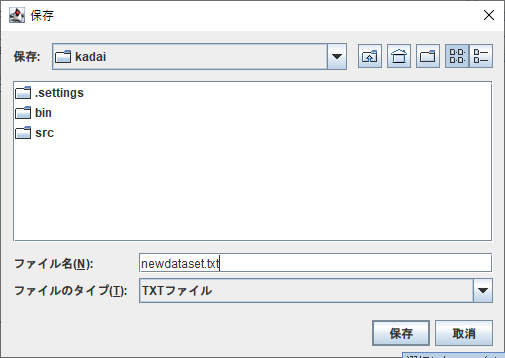
\includegraphics[bb=0 0 505 358,width=1\linewidth]{pic7.png}
  \caption{保存}
  \label{fig:pic7}
\end{figure}

\subsection{考察-29114007 池口 弘尚}
前回に引き続き、swingでGUIを作成した。

今回のプログラムの実装では、前回のものよりも出来ることの選択肢が増えているため、操作をGUI化することによって大きな恩恵を受けることができるように思われる。
コマンドで実行することを考えるとかなり操作が複雑化しそうなところを上手く簡単化できたと思う。
それぞれの操作をパネルで分けることによって、操作の切り替えが分かりやすくなるようにしている。
ただ、コマンドではエンターを押すだけで操作を進めることができたが、GUIではそれを行うことができない。


\section{感想-29114007 池口 弘尚}
GUIを作成するのは2度目のため、実装にそれほど時間はかからなかった。
そのため、発展ではない課題にも取り組んだが、勝手に進めていってしまったため、他のメンバーがするべき作業を取ってしまったように思う。
また、データベースクラスの仕様をしっかり決めずに実装に取り組んでしまったため、チームメイトがそれを利用したプログラムを書くのが遅くなってしまった。
そのため、わかる範囲でメソッドの仕様の共有をする必要があると思った。
\section{感想-29114031 大原 拓人}
時間が足りなくて、構造化したパターンを解析するプログラムまではできなかった。
はじめは複数パターンの照合を多重のforループで書こうとしていたが、ループの層の数がパターンの
数によって変わるので、再帰アルゴリズムが必要だと思い付いた。
再帰アルゴリズムのためには、メソッドのコールごとに変数を保持して、
そのコピーを引数で渡していくのだが、当初はデータベースの絞り込んだ結果の
配列のポインタも引数として渡そうとしていたので、読みづらいコードに
なっていたが、クラスのstatic変数を用いることで引数に含めなくてもよくなった。
あらためて、クラスの使い方を確認できた。


% 参考文献
\begin{thebibliography}{99}
	\bibitem{pl} prologのプログラムや挙動を参考にした
	\bibitem{swing} Swingを使ってみよう - Java GUIプログラミング
	\url{https://www.javadrive.jp/tutorial/} (2019年10月7日アクセス).
\end{thebibliography}

\end{document}